%!TEX root = ../terrainbook.tex

\setchapterpreamble[u]{\margintoc}


\graphicspath{{kriging/}}

\chapter{Spatial interpolation: kriging}%
\label{chap:kriging}

Kriging is a spatial interpolation method that was developed mostly by Georges Matheron based on the earlier work of Danie Krige, who created it to estimate the yield of gold mines in South Africa.
In contrast to other spatial interpolation methods, it involves creating a custom model that is fine-tuned using the statistical properties of each dataset.
In this way, kriging takes into account the specific characteristics of a dataset, often yielding better results than other interpolation methods.

Like other techniques based on geostatistical models, kriging relies on the fact that when one moves across space, values such as the gold content in rock or the elevation in a terrain have both a general spatial \emph{trend}\marginnote{trend}\index{trend} (\eg\ a flat mean value, a fitted plane or a more complex polynomial defining a surface) and a certain spatially correlated \emph{randomness} (\ie\ closer points tend to have more similar values).
Both of these elements are modelled in kriging.

More than a single method, kriging comprises a family of related methods.
Within this chapter, we will look at three related types of kriging.
These treat the spatially correlated randomness in a similar way, but they make different assumptions about the trend in a dataset.
These are:
\begin{itemize}
\item \emph{simple kriging}, where the trend is a known constant that is put into the model;
\item \emph{ordinary kriging}, where the trend is an unknown constant that we calculate in the interpolation process; and
\item \emph{universal kriging}, where we model the trend using a function.
\end{itemize}

\section{Statistical background}

The physical processes that shape the world can be considered to be at least partly deterministic.
In the case of a DTM, the elevation is determined by processes that we can model (more or less accurately), such as plate tectonics, volcanic activity and erosion.
However, these processes are much too complex and not well-enough understood to use them to obtain accurate elevation values.
Imagine, for instance, how difficult it would be to get an accurate elevation map of the world using only the shape of the tectonic plates and some other parameters (\eg\ their direction and speed of movement).

Because of this complexity, the value of complex properties, such as the elevation of a terrain, are usually treated in geostatistics as the result of what is known as a \emph{random}\marginnote{random process}\index{random process} or \emph{stochastic process}\marginnote{stochastic process}\index{stochastic process}.
In this context, randomness can be understood as the fact that the value of a property at an unsampled location is not known exactly, and so we cannot assign it an exact number.
Instead, the value at that location can be represented using statistics using a \emph{probability distribution}\marginnote{probability distribution}\index{probability distribution}, which we can associate with a function (\ie\ a \emph{probability distribution function}) or with a set of standard statistical measures, such as the mean and variance.

This situation is phrased in mathematical terms by saying that the value of the elevation property \(Z\) at a location \(x\) is a \emph{random variable}\marginnote{random variable}\index{random variable} \(Z(x)\).
For the sake of simplicity, we will usually omit the location and denote it just as \(Z\); or when working with multiple locations (\eg\ \(x_i\) and \(x_j\)), we will shorten their respective random variables (\(Z(x_i)\) and \(Z(x_j)\)) using subscripts (\(Z_i\) and \(Z_j\)).

In geostatistics, the most common way to express the general shape of the probability distribution of a random variable is in terms of its mean and its variance.
Here, the mean\marginnote{mean}\index{mean}, \emph{expectation}\marginnote{expectation}\index{expectation} or \emph{expected value}\marginnote{expected value}\index{expected value} of a random variable \(Z\) is a sort of probability-weighted average of its possible values and is denoted as \(E[z]\) or \(\mu\).
Meanwhile, the \emph{variance}\marginnote{variance}\index{variance} of a random variable \(Z\) is a measure of how far the values of \(Z\) will usually spread from its mean, and it is denoted as \(\mathrm{var}(Z)\) or \(\sigma^2\).
A small variance thus means that a few random samples of \(Z\) at nearby locations will likely form a tight cluster around its mean, whereas a large variance will have sample values that are more distant from the mean value.

Mathematically, the variance is defined as the expected value of the squared deviation from the expected value of \(Z\), or:

\begin{align}
\mathrm{var}(Z) &= E\left[{\left(Z-E\left[Z\right]\right)}^2\right] \label{eq:variance1} \\
&= E\left[Z^2 -2ZE\left[Z\right] + E[Z]^2\right] \nonumber \\
&= E\left[Z^2\right] - 2E\left[Z\right]E\left[Z\right] + E\left[Z\right]^2 \nonumber \\
&= E\left[Z^2\right] - 2E\left[Z\right]^2 + E\left[Z\right]^2 \nonumber \\
&= E\left[Z^2\right]-{E[Z]}^2. \label{eq:variance2}
\end{align}

Next, it is important to define the covariance\marginnote{covariance}\index{covariance}, denoted as \(\mathrm{cov}(Z_i,Z_j)\), or \(\sigma_{ij}\), which expresses the joint variability of the random variables \(Z_i\) and \(Z_j\).
Thus, a positive covariance between \(Z_i\) and \(Z_j\) means that when one increases or decreases, the other is expected to increase/decrease in the same direction.
Conversely, a negative covariance means that the variables tend to increase/decrease in opposite directions.
The magnitude of the covariance is related to the magnitude of this increase or decrease.
It is thus defined mathematically as the expected product of their deviations from their (individual) expected values, or:

\begin{align}
\mathrm{cov}(Z_i, Z_j) &= E\left[\left(Z_i-E[Z_i]\right) \left(Z_j-E[Z_j]\right)\right] \label{eq:covariance} \\
&= E\left[Z_iZ_j - Z_iE\left[Z_j\right] - E\left[Z_i\right]Z_j + E\left[Z_i\right]E\left[Z_j\right]\right] \\
&= E\left[Z_iZ_j\right] - E\left[Z_i\right]E\left[Z_j\right] - E\left[Z_i\right]E\left[Z_j\right] + E\left[Z_i\right]E\left[Z_j\right] \\
&= E\left[Z_iZ_j\right] - E\left[Z_i\right]E\left[Z_j\right]. \label{eq:covariance2}
\end{align}

Here, it is good to note that the covariance of \(Z_i\) with itself is equivalent to its variance:

\begin{equation}
\mathrm{cov}(Z,Z) = E\left[\left(Z-E[Z]\right)^2\right] = \mathrm{var}(Z). \nonumber
\end{equation}

While not used further in this lesson, it is also good to know that the variance and the covariance can be used to calculate the Pearson correlation coefficient\marginnote{correlation coefficient}\index{correlation coefficient} \(\rho_{ij}\), which is one of the most common statistical measures that is applied to datasets:

\begin{equation}
\rho_{ij}=\frac{\mathrm{cov}(Z_i, Z_j)}{\sqrt{\mathrm{var}(Z_i) \mathrm{var}(Z_j)}}. \nonumber
\end{equation}

Note that this is essentially just a normalised form of the covariance.

\section{Geostatistics and the standard geostatistical model}[Geostatistical model]

In geostatistics, we apply the concepts covered in the previous section on general-purpose statistics to also consider spatial phenomena, where values have a location and are often spatially correlated.

The model most commonly applied in geostatistics considers that a random variable \(Z\), which represents a spatially correlated property at a given location, can be decomposed into two related variables: (i) a non-random spatial trend that can be modelled by the expectation \(E[Z]\) (\eg\ using a constant, a polynomial, a spline, etc.); and (ii) a random but spatially correlated deviation from this trend that is considered as a sort of adjustment, error or residual term and is here denoted as \(R\).
In the case of elevation, the former would represent the general shape of the terrain, whereas the latter would represent local differences from it.
We therefore have:

\begin{equation}
\label{eq:geostat}
Z = E\left[Z\right] + R.
\end{equation}

It is important to consider a couple important aspects here.
First, note that since \(R = Z - E[Z] \), the variance (Equation~\ref{eq:variance1}) and covariance (Equation~\ref{eq:covariance}) can also be defined in terms of the residuals:

\begin{align}
\mathrm{var}\left(Z\right) &= E\left[{R}^2\right], \label{eq:varres} \\
\mathrm{cov}(Z_i,Z_j) &= E\left[R_i \cdot R_j\right]. \label{eq:covres}
\end{align}

Also, it is important to know that since the expectation is by definition the mean, in order not to introduce any bias, the expected value of the residual must be zero.
That is, \(E\left[R\right] = 0\).

\section{The variogram}%
\index{variogram}

As we saw in simple kriging, the theoretical definitions of the variance and covariance functions imply that we know the expected value (\ie\ \(E[Z]\) in Equation~\ref{eq:variance1}, and \(E[Z_i]\) and \(E[Z_j]\) in Equation~\ref{eq:covariance}), which in practice is not realistic.
In order to avoid this problem, most other forms of kriging rely instead on what is known as a \emph{variogram}.
The variogram \(\gamma(h)\) is a function that expresses the average dissimilarity of the value of a random variable \(Z\) between sample points at different distances.
It is defined as:

\begin{equation}
\gamma(h) = \frac{1}{2} (Z(x+h) - Z(x))^2,
\end{equation}

where \(x\) is a sample point, \(h\) is a vector from \(x\) to another sample point and \(Z(x)\) is the value of a random variable at \(x\) (\eg\ its elevation).

When this is done with every possible pair of sample points in a dataset, or with a representative subset in order to speed up the process as it is usually done in practice, \(|h|\) (\ie\ the magnitude of the vector \(h\)) and \(\gamma(h)\) can be put into a scatter plot to show how the average dissimilarity of a value changes with the distance between the sample points.
The result of such a plot is what is known as a \emph{variogram cloud}\marginnote{variogram cloud}\index{variogram cloud} (Figure~\ref{fig:variogram_cloud}).

\begin{figure*}
\begin{subfigure}{0.5\linewidth}
\centering
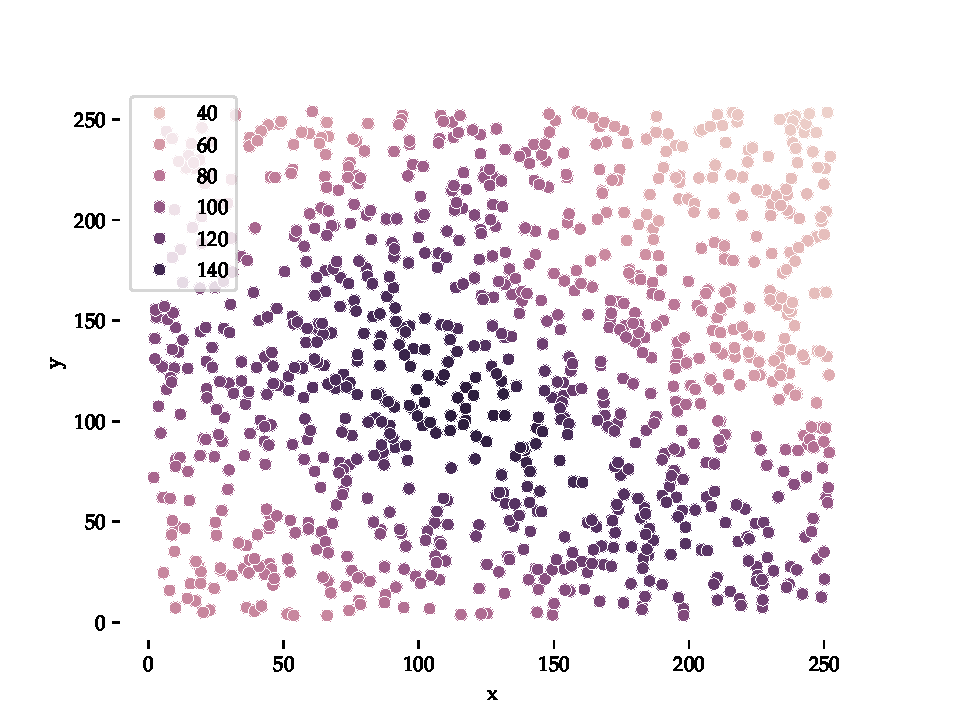
\includegraphics[width=\linewidth]{figs/data}
\caption{dataset}
\end{subfigure}%
\begin{subfigure}{0.5\linewidth}
\centering
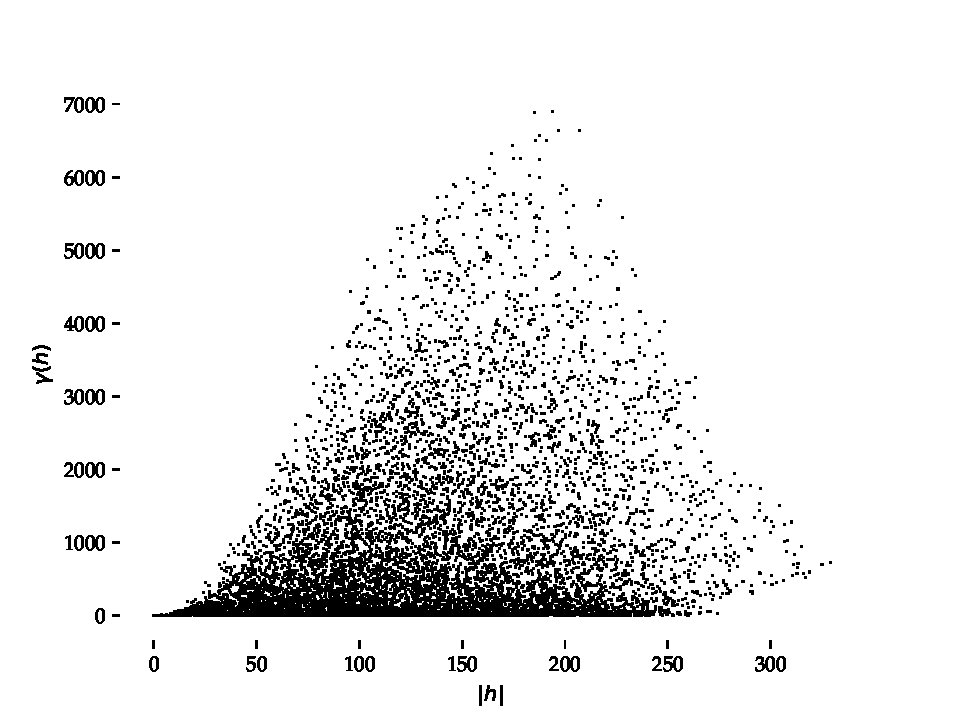
\includegraphics[width=\linewidth]{figs/variogram_cloud}
\caption{variogram cloud}
\end{subfigure}%
\caption{Starting from (a) a sample dataset, (b) the variogram cloud can be computed.
In this case, only 1\% randomly selected point pairs were used.}%
\label{fig:variogram_cloud}
\end{figure*}

In this figure, it is possible to see some typical characteristics of a variogram cloud.
Since nearby sample points tend to have similar values, the dissimilarity tends to increase as the distance between sample points increases.
However, it is worth noting that since the farthest away pairs of sample points have similar values in this specific dataset, the dissimilarity also decreases at the highest distances.

Since most of the time there is a wide variation between the dissimilarities shown at all distances in a variogram cloud, the next step is to average the dissimilarity of the pairs of sample points based on distance intervals.
Mathematically, a series of averages of dissimilarities \(\gamma^\star(h)\) can be created by computing the average dissimilarities for all vectors whose lengths are within a series of specified intervals (generally known as \emph{bins}).
Given a set \(\mathfrak{h}\) containing the vectors for a length interval, the average for its dissimilarity class is computed as:

\begin{equation}
\gamma^\star(\mathfrak{h}) = \frac{1}{2n}\sum\left(z\left(x+h\right)-z\left(x\right)\right)^2 \hspace{1cm}\text{for all } h \in \mathfrak{h}
\end{equation}

where \(n\) is the number of sample point pairs in \(\mathfrak{h}\).

This computation results in much smoother values for the dissimilarity, and when the results of \(|h|\) and \(\gamma^\star(h)\) are put into a scatter plot (Figure~\ref{fig:experimental_variogram}), the result is what is known as an \emph{experimental variogram}\marginnote{experimental variogram}\index{experimental variogram}.
Experimental variograms are based on a few parameters (Figure~\ref{fig:experimental_variogram}b illustrates these): 
\begin{itemize}
  \item the \emph{sill}\marginnote{sill}\index{sill}, which is the upper bound of \(\gamma^\star(h)\);
  \item the \emph{range}\marginnote{range}\index{range}, which is the value of \(|h|\) when it converges; 
  \item the \emph{nugget}\marginnote{nugget}\index{nugget}, which is the value of \(\gamma^\star(h)\) when \(|h| = 0\).
\end{itemize}
Note that in order to avoid the unreliable dissimilarities that are common at large distances between sample points, it is usual practice to only compute the experimental variogram for distances up to half of the size of the region covered by the dataset.

\begin{figure*}
\begin{subfigure}{0.5\linewidth}
\centering
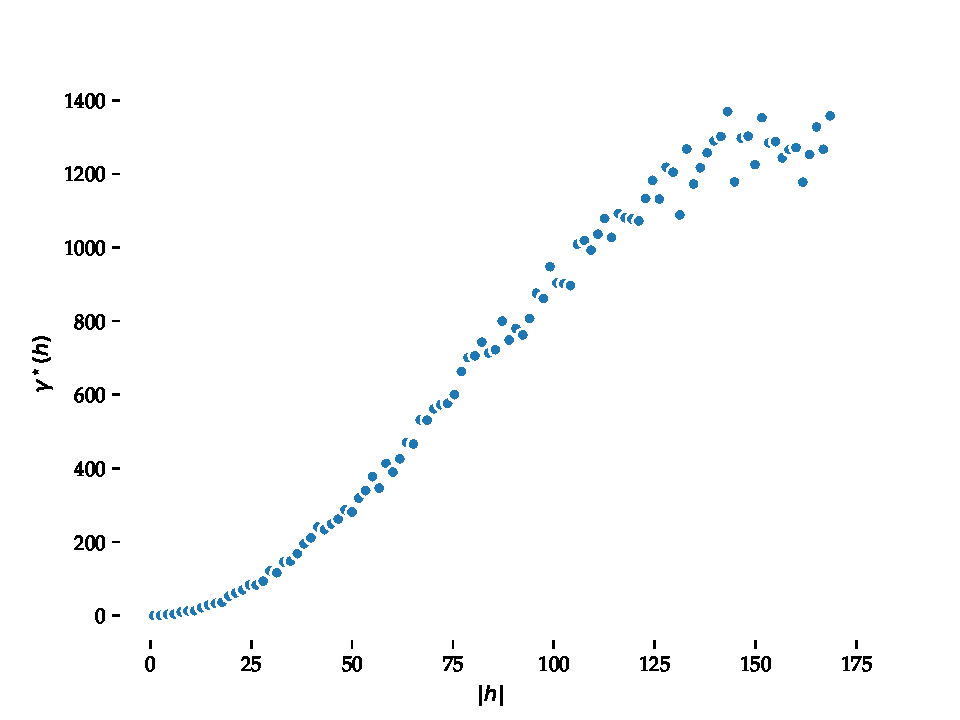
\includegraphics[width=\linewidth]{figs/experimental_variogram}
\caption{experimental variogram}
\end{subfigure}%
\begin{subfigure}{0.5\linewidth}
\centering
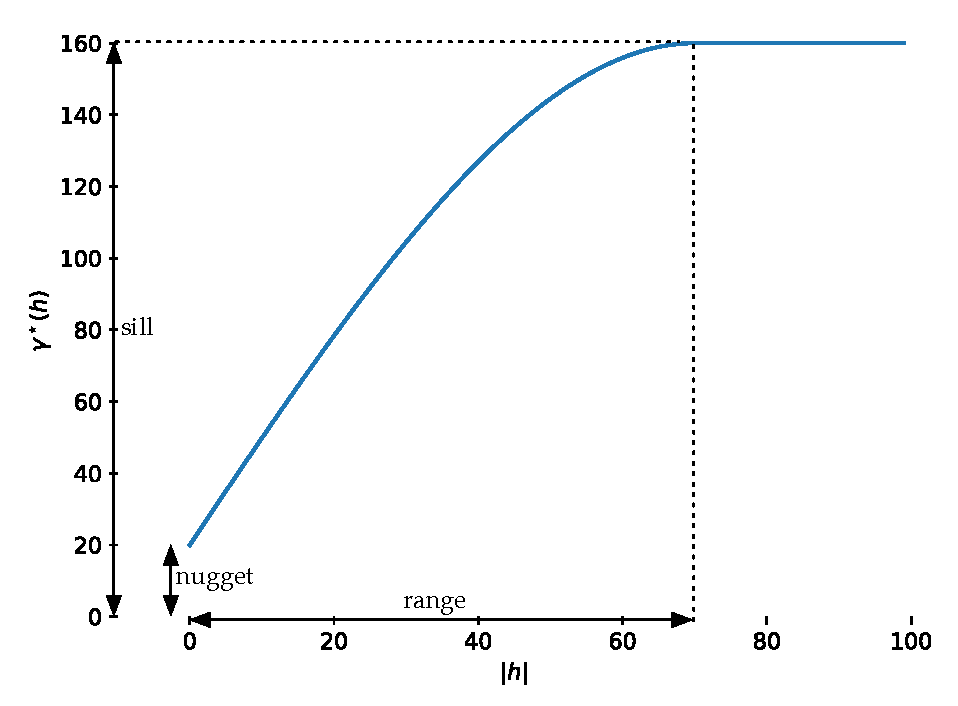
\includegraphics[width=\linewidth]{figs/example_variogram}
\caption{parameters}
\end{subfigure}%
\caption{(a) The experimental variogram is usually described in terms of (b) its parameters.}%
\label{fig:experimental_variogram}
\end{figure*}

Finally, the last step is to replace the experimental variogram with a \emph{theoretical variogram function}\marginnote{theoretical variogram function}\index{theoretical variogram function} that approximates it and which can be more easily evaluated for further calculations.
Depending on the shape of the variogram, there are various functions that can be used.
Some examples are:

\begin{align}
\gamma_\mathrm{exponential}(h) &= s \left(1 - e^\frac{-3|h|}{r}\right) + n \\
\gamma_\mathrm{gaussian}(h) &= s \left(1 - e^\frac{-\left(3|h|\right)^2}{r^2}\right) + n \\
\gamma_\mathrm{spherical}(h) &= \begin{cases} 
   s \left(\frac{3|h|}{2r} - \frac{|h|^3}{2r^3}\right) + n & \text{if } |h| \leq r \\
   s + n & \text{if } |h| > r
  \end{cases}
\end{align}

where \(s\) is the \emph{sill}, set to roughly the value of \(\gamma^\star(h)\) when \(\gamma^\star(h)\) is  flat; \(r\) is the \emph{range}, roughly the minimum value of \(|h|\) where \(\gamma^\star(h)\) is flat, and \(n\) is the nugget, which is the starting value of \(\gamma^\star(h)\).
Figure~\ref{fig:theoretical_variogram} shows the result of fitting the three example theoretical variogram functions, exponential, Gaussian and spherical.
Note how the Gaussian function appears to be a better fit in this case.

\begin{figure}[htbp]
\centering
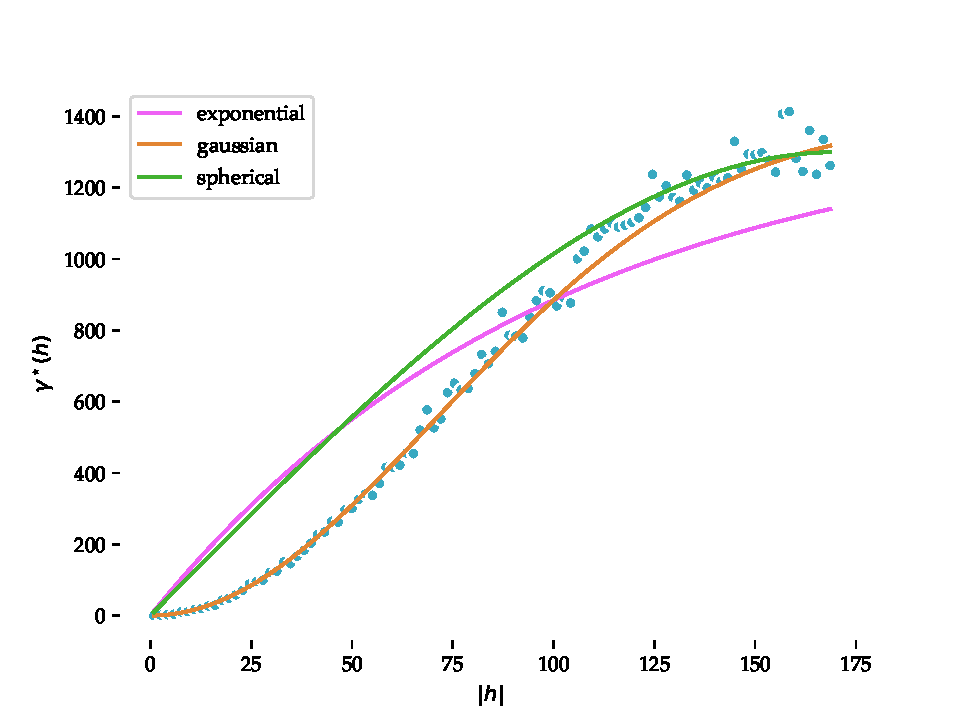
\includegraphics[width=0.8\linewidth]{figs/theoretical_variogram}
\caption{Three possible theoretical variogram functions}%
\label{fig:theoretical_variogram}
\end{figure}

These functions can be used as covariance functions for simple kriging, taking into account that \(\gamma(h) = C(0) - C(h)\).
Note that this means that the covariance is high when \(|h|\) is small and it decreases as \(|h|\) increases.

\section{Simple kriging}

Simple kriging starts from the assumption that in the geostatistical model from Equation~\ref{eq:geostat}, the expectation \(E(Z)\) is the same everywhere, which is known as the \emph{stationarity of the mean}\marginnote{stationarity of the mean}\index{stationarity of the mean}, and that it is \emph{known}.
In the case of a DTM, that would mean that a terrain might be uneven with significant peaks and valleys, but that there is not a general trend across it (\eg\ a clear slope with higher elevations on one side and lower elevations on the opposite side).
Mathematically, we can express that as:

\begin{align}
\label{eq:expectationsk}
E\left[Z(x+h\right)] = E\left[Z(x)\right],
\end{align}

where \(x\) is an arbitrary point in the domain (\ie\ the area we want to interpolate), \(h\) is any vector from \(x\) to another point in the domain and \(Z(x)\) is the value of a random variable at \(x\) (\eg\ its elevation).

Next, simple kriging also makes the assumption that the covariance between a random variable at a pair of locations does not depend on the locations, but instead can be defined based only on the vector separating them.
In the case of a DTM, this would mean that the likelihood of finding similar elevations at two points separated by a given distance and orientation does not change across the terrain.
For instance, a terrain that goes from smooth on one side to rough on the other would not satisfy this assumption.
Mathematically, we can express this as:

\begin{align}
\label{eq:covariancesk}
\mathrm{cov}\left(Z(x+h), Z(x)\right) = C(h),
\end{align}

where \(C\) is the covariance function.
Since both the expectation (Equation~\ref{eq:expectationsk}) and the covariance (Equation~\ref{eq:covariancesk}) are translation invariant, this pair of assumptions are together known as \emph{second-order stationarity}\marginnote{second-order stationarity}\index{second-order stationarity}.

Simple kriging is similar to the other spatial interpolation methods that use a weighted average.
However, since we are assuming that the expectation is the same everywhere, we will define it as a weighted average of residuals \(R\) of the form \(Z-E[Z]\), after which the expectation needs to be added back in order to obtain the final value.
It thus defines a function \(\hat{R}_0\) that estimates the value of the residual \(R\) of the random variable \(Z\) at a location \(x_0\) as a weighted average of its residuals at the \(n\) sample points \(x_i\) that we will use for the interpolation (where \(1 \leq i \leq n\)).
We denote this as:

\begin{equation}
\label{eq:wask}
\hat{R}_0 = \hat{Z}_0 - E[Z_0] = \sum_{i=1}^n w_i (\underbrace{Z_i-E[Z_i]}_{R_i}).
\end{equation}

Kriging has two distinguishing characteristics.
First, that it is \emph{unbiased}\marginnote{unbiased}\index{unbiased}.
This means that it creates a model where the expected value of the estimation at a location \(x_0\) is equal to the expected value at that location.
In mathematical terms, we can formulate this as:

\begin{equation}
\label{eq:unbiased}
E\left[ \hat{Z}_0 - Z_0 \right] = 0 \hspace{1cm}\text{or}\hspace{1cm}E\left[Z_0\right] = E\left[ \hat{Z}_0 \right].
\end{equation}

In order to check this for simple kriging, we can put the weighted average from Equation~\ref{eq:wask} in this equation, which results in the following:

% TODO : why is latex complaining at \end{align} I removed \cancelto{} and it's solved
\begin{align}
  E\left[ Z_0 \right] &= E\left[ E[Z_0] + \sum_{i=1}^n w_i R_i \right] \nonumber \\
  &= E[Z_0] + \sum_{i=1}^n w_i 0{E[R_i]} \nonumber \\
  &= E[Z_0].  \nonumber
\end{align}

The second property of kriging is that it \emph{minimises the variance of the estimation error}\marginnote{minimisation of the variance}\index{minimisation of the variance}, which in this case is given by \(\mathrm{var}\left(\hat{R}_0 - R_0\right)\).
If we use the definition of the variance from Equation~\ref{eq:variance1}, this can be instead put in terms of an expectation:

\begin{equation}
\mathrm{var}\left(\hat{R}_0 - R_0\right) = E \left[ \left( \left(\hat{R}_0 - R_0\right) - E \left[\hat{R}_0 - R_0\right] \right)^2 \right] \nonumber
\end{equation}

However, we know from the unbiased criterion from Equation~\ref{eq:unbiased} that \(E\left[ \hat{R}_0 - R_0 \right] = 0\), and so we can simplify the previous equation as:

\begin{equation}
\mathrm{var}\left(\hat{R}_0 - R_0\right) = E\left[\left( \hat{R}_0 - R_0 \right)^2\right] \nonumber.
\end{equation}

If this is expanded, it results in:

\begin{align}
\mathrm{var}\left(\hat{R}_0 - R_0\right) &= E\left[{\hat{R}_0}^{\hspace{1.2mm}2} - 2\hat{R}_0R_0 + {R_0}^2 \right] \nonumber \\
&= E\left[{\hat{R}_0}^{\hspace{1.2mm}2}\right] - 2E\left[\hat{R}_0R_0\right] + E\left[{R_0}^2 \right] \nonumber \\
&= E\left[\sum_{i=1}^n \sum_{j=1}^n w_i w_j R_i R_j\right] - 2E\left[\sum_{i=1}^n w_i R_i R_0\right] + E\left[{R_0}^2 \right] \nonumber \\
&= \sum_{i=1}^n \sum_{j=1}^n w_i w_j E\left[R_i R_j\right] - 2\sum_{i=1}^n w_i E\left[R_i R_0\right] + E\left[{R_0}^2 \right]. \nonumber
\end{align}

Here, we can use the definitions of the variance based on residuals from Equations~\ref{eq:varres} and~\ref{eq:covres} together with our covariance formula from Equation~\ref{eq:covariancesk}, which yields:

\begin{align}
\mathrm{var}\left(\hat{R}_0 - R_0\right) &= \sum_{i=1}^n \sum_{j=1}^n w_i w_j \mathrm{cov}(R_i, R_j) - 2\sum_{i=1}^n w_i \mathrm{cov}(R_i,R_0) + \mathrm{cov}(R_0, R_0) \label{eq:variancesk} \\
&= \sum_{i=1}^n \sum_{j=1}^n w_i w_j C(x_i-x_j) - 2\sum_{i=1}^n w_i C(x_i-x_0) + C(x_0-x_0).
\end{align}

In order to minimise this equation, we can find where its first derivative is zero.
This is:

\begin{equation}
\frac{\partial \mathrm{var}\left(\hat{R}_0 - R_0\right)}{\partial w_i} = 2 \sum_{j=1}^n w_j C(x_i-x_j) - 2C(x_i-x_0) = 0 \hspace{1cm} \text{for all } 1 \leq i \leq n, \nonumber
\end{equation}

which yields the set of \(n\) simple kriging equations:

\begin{equation}
2 \sum_{j=1}^n w_j C(x_i-x_j) = 2C(x_i-x_0).
\end{equation}

While these equations can be used to perform simple kriging, it is often easier to deal with these in matrix form:

\begin{equation}
%
\underbrace{\left( \begin{array}{ccc}
C(x_1-x_1) & \cdots & C(x_1-x_n) \\
\vdots & \ddots & \vdots \\
C(x_n-x_1) & \cdots & C(x_n-x_n) \end{array} \right)}_{A}
%
\underbrace{\left(\begin{array}{c}
w_1 \\
\vdots \\
w_n \end{array} \right)}_{w} = 
%
\underbrace{\left(\begin{array}{c}
C(x_1-x_0) \\
\vdots \\
C(x_n-x_0) \end{array} \right)}_{d}
\end{equation}

which is known as the \emph{simple kriging system}\marginnote{simple kriging system}\index{simple kriging system}.
Finally, if we invert the matrix \(A\), the interpolation weights are given by:

\begin{equation}
w = A^{-1}d.
\end{equation}

Now, the obvious remaining questions are: (i) what expectation \(E[Z]\) to use, and (ii) what covariance function \(C\) to use.
Without an external evaluation of the dataset, there are no optimal answers for either of those questions, which is the main weakness of simple kriging and the reason why it is not used widely in practice.
That being said, a reasonable solution could be to use the average value of \(z_i\) for all points as \(E[Z]\), and an arbitrary covariance function, such as the exponential, Gaussian and spherical functions that we discuss in the following section.

\section{Ordinary kriging}%
\index{ordinary kriging}

Ordinary kriging is similar to simple kriging and to other spatial interpolation methods that use a weighted average (see Equation~\ref{eq:wask}).
It thus defines a function \(\hat{Z}_0\) that estimates the value of the random variable \(Z\) at a location \(x_0\) as a weighted average of its value at the \(n\) sample points \(x_i\) that we will use for the interpolation (where \(1 \leq i \leq n\)).
We denote this as:

\begin{equation}
\label{eq:waok}
\hat{Z}_0 = \sum_{i=1}^n w_i Z_i.
\end{equation}

Like simple kriging, ordinary kriging is \emph{unbiased}.
This means that it creates a model where the expected value of the estimation at a location \(x_0\) is equal to the expected value at that location.
In practice, this means that if we put the weighted average from the previous equation in Equation~\ref{eq:unbiased}, it results in the following:

\begin{equation}
E\left[ Z_0 \right] = E\left[ \sum_{i=1}^n w_i Z_i\right] = \sum_{i=1}^n w_i E\left[Z_i\right].
\end{equation}

Here, \emph{ordinary kriging} also makes the assumption that the expectation is the same everywhere (stationarity of the mean).
Therefore, \(E\left[Z_i\right]\) has the same value everywhere (\ie\ it is a constant) and we can thus move it outside of the summation:

\begin{equation}
E\left[ Z_0 \right] = E\left[Z_i\right] \sum_{i=1}^n w_i,
\end{equation}

and since also \(E\left[Z_i\right] = E\left[ Z_0 \right] \) (because of the stationarity of the mean), the two terms cancel each other out in the previous equation, which means that the unbiased property in ordinary kriging implies that the interpolation weights must add up to one:

\begin{equation}
\sum_{i=1}^n w_i = 1.
\end{equation}

Fulfilling this criterion means that we can use the variogram in ordinary kriging, which is not true for simple kriging.

Like simple kriging, ordinary kriging \emph{minimises the variance of the estimation error}, which is given by \(\mathrm{var}\left(\hat{Z}_0 - Z_0\right)\).
For this, we can use the same derivation as for simple kriging up to Equation~\ref{eq:variancesk} but using the variogram for the final step.
This is:

\begin{align}
\mathrm{var}\left(\hat{R}_0 - R_0\right) &= \sum_{i=1}^n \sum_{j=1}^n w_i w_j \mathrm{cov}(R_i, R_j) - 2\sum_{i=1}^n w_i \mathrm{cov}(R_i,R_0) + \mathrm{cov}(R_0, R_0) \nonumber \\
&= -\sum_{i=1}^n \sum_{j=1}^n w_i w_j \gamma(x_i-x_j) + 2\sum_{i=1}^n w_i \gamma(x_i-x_0) - \gamma(x_0-x_0).
\end{align}

Using the previous equation and the unbiased criterion from Equation~\ref{eq:unbiased}, we can apply the minimisation method known as Lagrange multipliers\footnote{\url{https://en.wikipedia.org/wiki/Lagrange_multiplier}} and arrive at the set of \(n+1\) ordinary kriging equations:

\begin{align}
\sum_{j=1}^n w_i \gamma(x_i-x_j) + \mu(x_0) &= \gamma(x_i - x_0) \hspace{1cm} \text{for all } 1 \leq i \leq n \nonumber \\
\sum_{j=1}^n w_i &= 1 
\end{align}

where \(\mu(x_0)\) is a Lagrange parameter that was used in the minimisation process.

Like with simple kriging, these equations can be used to perform ordinary kriging, but it is often easier to deal with these in matrix form:

\begin{equation}
%
\underbrace{\left( \begin{array}{cccc}
\gamma(x_1-x_1) & \cdots & \gamma(x_1-x_n) & 1 \\
\vdots & \ddots & \vdots & 1 \\
\gamma(x_n-x_1) & \cdots & \gamma(x_n-x_n) & 1 \\
1 & \cdots & 1 & 0 \end{array} \right)}_{A}
%
\underbrace{\left(\begin{array}{c}
w_1 \\
\vdots \\
w_n \\
\mu(x_0) \end{array} \right)}_{w} = 
%
\underbrace{\left(\begin{array}{c}
\gamma(x_1-x_0) \\
\vdots \\
\gamma(x_n-x_0) \\
1 \end{array} \right)}_{d}
\end{equation}

which is known as the \emph{ordinary kriging system}\marginnote{ordinary kriging system}\index{ordinary kriging system}.

Finally, if we invert the matrix \(A\), the weights and the Lagrange multipliers are given by:

\begin{equation}
w = A^{-1}d
\end{equation}

\section{Universal kriging}%
\index{universal kriging}

%%%
%
\section{Implementation}

Kriging can be directly applied to any point on the plane, yielding a result such as the one in Figure~\ref{fig:interpolation}.
However, much like other interpolation methods, kriging is only reliable in the domain (\ie\ roughly the convex hull of the points).
It can extrapolate (often with negative weights), but that does not mean that the results outside the domain are accurate.

\begin{figure}[htbp]
\centering
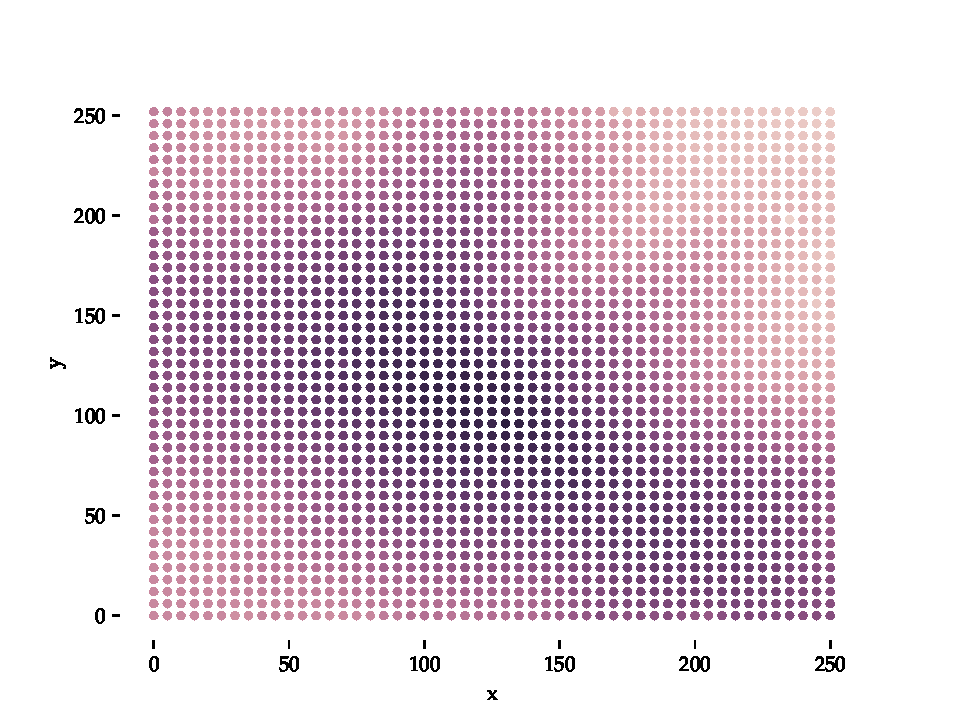
\includegraphics[width=\linewidth]{figs/interpolation}
\caption{The result of using ordinary kriging to interpolate on a grid of points using the sample dataset using only the sample points within 15 units of each interpolated point.}%
\label{fig:interpolation}
\end{figure}

Finally, it is also important to consider some computational aspects into account.
If a large number of sample points are used to interpolate every point, kriging can be \emph{very slow}.
The reason for this is because matrix \(A\) will be very large, and inverting a matrix is a computationally expensive process.
However, inverting very large matrices is not really needed in practice.
When a sample point is far from the interpolated point, its weight will be low, and it will thus have only a small influence on it.
Because of this, it is usually best to only take into account a few sample points in the calculation, either by limiting the sample points to those within a given search radius, or by selecting only a given number of its closest sample points.
However, you should note that this can cause artefacts in the final result.

%%%
%
\section{Notes and comments}

\citet{Krige51} is the original publication by Danie Krige, which was later formalised by Georges Matheron~\citep{Matheron62,Matheron65}.
How this came to be is best explained in \citet{cressie93}.

If you have trouble following the derivations of the kriging equations or want to know more about them, \citet{Lichtenstern13} explains this well.
If you feel like your statistics background is a bit weak, you first might want to have a look at \citet{Fewster14}, particularly Chapter~3.

A relatively simple explanation of Kriging with agricultural examples is given by \citet{Oliver15}.
A standard reference textbook that is good but not so easy to follow is \citet{Wackernagel03}.

such as the specific spatial correlation between the points in the dataset or their highly unequal distributions of sample points


different characteristics that are specific to a dataset, such as , anisotropy (spatial correlation that varies according to a direction), or the varying uncertainty and spatial correlation of a set of sample points (eg when measurements are taken with different instruments/techniques).

Two other good Youtube videos that explain kriging:
\begin{itemize}
\item \url{https://www.youtube.com/watch?v=CVkmuwF8cJ8}
\item \url{https://www.youtube.com/watch?v=98zz25kTteQ}
\end{itemize}

%%%
%
\section{Exercises}

\begin{enumerate}
\item Why can using a search radius create artefacts in the interpolated terrain?
\item If kriging generally provides better results than other interpolation methods, why would you use something else (eg IDW)?
\item What does a nugget of zero say about a dataset? What about a large nugget?
\item What kind of dataset would yield a flat variogram (\ie\ a horizontal line)?
\end{enumerate}